\subsection{The Static Algorithm}
\label{sec:static}

We will end with an outline of the static algorithm first investigated in works \cite{dang2012reachability, dreossi2016parallelotope}. As mentioned in the previous section, the building block of the reachability algorithm relies on approximate solutions to a non-linear optimization problem over the unitbox domain. Consider a non-linear function $h : \reals^n \rightarrow \reals$. The most general form of this optimization problem can be expressed as:
%
\begin{eqnarray}
  \max ~ h(x) \label{eq:maxsup}\\
  s.t. ~~ x \in [0,1]^{n}.\nonumber
\end{eqnarray}

In the static algorithm, the user manually specifies the number of parallelotopes and a set of static directions for each parallelotope. In other words, the user must specify the template matrix $\Lambda$ and its corresponding offset vector $c$ for each parallelotope $P = \langle \Lambda, c\rangle$ contained in the bundle \emph{before} the computation begins.

We now proceed to formally describe the static algorithm.
%
First, a small remark on the template matrix of the parallelotopes $P_i$ contained in some bundle $Q$. It is possible that some of the parallelotopes share the same template matrix directions.
%
 In other words, for $P_i = \langle \Lambda^{P_i}, c^{P_i} \rangle, P_j = \langle \Lambda^{P_j}, c^{P_j} \rangle$ such that $P_i, P_j \in \ptopeset{Q}$, there could exist some $k$ such that $\Lambda^{P_i}_k = \Lambda^{P_j}_k$ as row vectors.
%
Thus, a more compact method of encoding the bundle is by taking the \emph{distinct} template directions as rows of a new template matrix $\Lambda^Q$ along with its corresponding offset vector $c^Q$.
%
To distinguish between the distinct parallelotopes contained in the bundle, we add a new matrix called the \emph{bundle index matrix}, $\T^Q \in \mathbb{N}^{p \times n}$, such that $\T^Q_i$ is a vector of row indices of $\Lambda^Q$ which specify the template directions defining parallelotope $P_i \in \ptopeset{Q}$.
%
The number of rows will thus be the number of distinct parallelotopes contained in the bundle $p = |\ptopeset{Q}|$.
%
\begin{remark}
If none of the paralleotopes $P_i \in \ptopeset{Q}$ share common template directions, then $\Lambda^Q$ will simply be the template direction matrices $\{\Lambda^P\}_{P \in \ptopeset{Q}}$ concatented along their rows. This will generally be the matrix generated by the dynamic algorithm we will outline in a future section.
\end{remark}
%
\begin{example}

\end{example}

Another input to the algorithm is the initial parallelotope bundle, given as $Q$. When the initial set is a box, $P_0$ will be defined by the axis-aligned template directions.

The output of the algorithm is, for each step $k$, the set $\overline\Theta_k$, which is an overapproximation of the reachable set at step $k$, $\Theta_k \subseteq \overline\Theta_k$. The total overapproximation of the reachable set for a finite number of steps $n$ will be $\Theta = \cup_{k=1}^n \Theta_k$.
%
The high-level pseudo-code is written in Algorithm~\ref{alg:old}.

The algorithm simply calls $\tbundle$ for each step, producing a new parallelotope bundle computed from the previous step's bundle.
%
To compute the image of $Q$, the algorithm computes the upper and lower bounds of $f(x)$ with respect to each template direction $\Lambda_i^Q$.
%
Since computing the maximum value of $f(x)$ along each template direction on the $Q$ in one shot is computationally difficult, the algorithm instead computes the maximum value over each of the constituent parallelotopes and uses the minimum of all these maximum values.

The $\tbundle$  operation works as follows.
%
Consider a parallelotope $P$ in the bundle $Q$.
%
% and half-space representation as $\tup{\T, c_{l}, c_{u}$.
Given a template direction $\Lambda_i^Q$, the maximum value of $\Lambda_{i}^Q f(x)$ for all $x \in Q$ is less than or equal to the maximum value of $\Lambda_{i}^P \cdot f(x)$ for all $x \in P$ such that $\Lambda_i^Q$ is a row in $\Lambda^P$.
%
Similar argument holds for the minimum value of $\Lambda_{i}^Q \cdot f(x)$ for all $x \in Q$.
%
Observe that these inequalities hold by virtue of the fact that $Q \subseteq P$ by definition.
%
To describe this more formally: if $\lambda^Q_i = \{ P \in \ptopeset{Q} ~|~ \Lambda_i^Q = \Lambda_k^P \text{ for some } k \}$, then
%
\begin{align}
    & \max_{x \in Q}{\Lambda_{i}^Q \cdot f(x)} \leq \min_{P \in \lambda^Q_i} {\max_{x \in P}{\Lambda_{i}^P \cdot f(x)}}  \label{eq:max_over_ptopes}
 \\
    & \max_{P \in \lambda^Q_i} {\min_{x \in P}{\Lambda_{i}^P \cdot f(x)}} \leq \min_{x \in Q}{\Lambda_{i}^Q \cdot f(x)} \label{eq:min_over_ptopes}
\end{align}

%
% We would like to compute the image of the parallelotope $P$ with respect to the non-linear transformation $f(x)$.
%
% That is, we would like to compute $P'$ such that $\forall x \in P, f(x) \in P'$.
%
% Given that current techniques use static template directions, the parallelotope $P'$ also uses the template directions $\T^{P}$.
%
To compute the upper and lower bounds of each template direction $\Lambda_{i} f(x)$, for all $x \in P$, we perform the following optimization.
%
\begin{eqnarray}
  \max ~ \Lambda_i^{P} \cdot f(x) \label{eq:maxf}\\
  s.t. ~~ x \in P.\nonumber
\end{eqnarray}
%
\noindent Note that $\Lambda_i^{P} \cdot f(x)$ is a dot product between the row vector $\Lambda_i^{P}$ and the component-wise dynamics of $f(x)$. This is similar to the method of computing support functions over convex sets \cite{boyd2004convex}.


By , all the states in $P$ can be expressed as a vector summation of an anchor and a convex combination of generators.
%
Let  $\langle v, g_1, \cdots, g_n \rangle$ be the generator representation of $P$.
%
The optimization problem given in Equation~\ref{eq:maxf} would then transform as follows.

\begin{eqnarray}
  \max ~ \Lambda_i^P \cdot f(a + \Sigma_{i=1}^{n} \alpha_i g_i) \label{eq:maxalpha}\\
  s.t. ~~ \overline\alpha \in [0,1]^{n}.\nonumber
\end{eqnarray}

Equation~\ref{eq:maxalpha} is a form of $\mathsf{optBox(\Lambda_{i} \cdot f)}$ over $[0,1]^n$.
%
One can compute an upper-bound to this non-linear optimization by computing the Bernstein coefficients of $\Lambda_i \cdot f(a + \Sigma_{i=1}^{n} \alpha_i g_i)$ and taking the maximum and minimum coefficients as shown in Property~\ref{prop:bern_enclosure}.
%
Similarly, we compute the lower-bound of $\Lambda_{i}\cdot f(x)$ for all $x \in P$ by computing the upperbound of $-1 \times \Lambda_{i}\cdot f(x)$.
%

We iterate this process (i.e., computing the upper and lower bound of $\Lambda^Q_{i}\cdot f(x)$) for each parallelotope in the bundle $Q$ according to Equation \ref{eq:max_over_ptopes} and Equation \ref{eq:min_over_ptopes}).
%
% Observe that the role of the parallelotopes in the bundle is to compute an upper bound on the maximum value of $T_{i}f(x)$ by expanding the domain from $Q$ to the corresponding parallelotope $P$.
%
Therefore, the tightest upper bound on $\Lambda^Q_{i}\cdot f(x)$ over $Q$ is the least of the upper bounds computed from each of the parallelotopes.
%
A similar argument holds for lower bounds of $\Lambda^Q_{i}\cdot f(x)$ over $Q$.
%
Therefore, the image of the bundle $Q$ will be the bundle $Q'$ where the upper and lower bounds for templates directions are obtained by solving a series of non-linear optimization problems of the form presented in Equation~\ref{eq:maxf}.

% TODO: Expound more on the menaings of constructing ptopes from the bundle index matrix.

Finally, once the loop on step two of Algorithm~\ref{alg:old} halts at step $S$, the outputted reachable set will be the computed over-approximations $\overline\Theta_1, \cdots, \overline\Theta_S$. As step four within the loop implies, this is simply the image bundles $Q'$ returned by our $\tbundle$ procedure.


%-----------------------------------------------------------------------------------------------------------------------------------------------------------------

\begin{figure}[t!]

\begin{algorithm}[H]
  \SetKwInput{KwInput}{Input}
  \SetKwInput{KwOutput}{Output}
  \SetKwFunction{AppendPCA}{AppendNewPCATemplates}
  \SetKwFunction{AppendLin}{AppendNewLinAppTemplates}
  \SetKwFunction{TransformBund}{TransformBundle}
  \SetKwFunction{UpdateTemp}{UpdateTemplates}
  \SetKwFunction{GetSupp}{GetSupportPoints}
  \SetKwFunction{PropPoints}{PropagatePointsOneStep}
  \SetKwFunction{PCA}{PCA}
  \SetKwFunction{ApproxLinearTrans}{ApproxLinearTrans}
  \SetKwFunction{SetLifeSpan}{SetLifeSpan}
  \SetKwFunction{AddTemptoBund}{AddTemplateToBundle}
  \SetKwFunction{RemoveTemp}{RemoveTempFromBund}
  \SetKwProg{Fun}{Proc}{:}{}

\SetAlgoLined
\DontPrintSemicolon

\KwInput{Dynamics $f$, Initial Parallelotope $P_0$, Step Bound $S$, Template Dirs $\Lambda$, indexes for parallelotopes $I$}
\KwOutput{Reachable Set Overapproximation $\overline\Theta_k$ for each step $k$}
$Q_0 = \{ P_0 \}$ \;
 \For{$k \in [1, 2, \ldots, S]$}{
    $Q_k$ = \TransformBund($f$, $Q_{k-1}$, $\Lambda$) \;
   $\overline\Theta_k = Q_k$ \;
 }
 \Return{$\overline\Theta_1 \ldots \overline\Theta_S$} \;
 \;
 %
 \Fun{\TransformBund{$f$, $Q$, $\Lambda$}}{
   $Q' \gets \{\}$; $c_{u} \gets +\infty$; $c_{l} \gets -\infty$\;
   \For{each parallelotope $P$ in $Q$}{
     % $\tup{\T, c_{l}, c_{u}} \gets \mathsf{half-spaceRepresentation}(P)$\;
     $\langle v, G \rangle \gets \mathsf{generatorRepresentation}(P)$\;
     \For{each template direction $\Lambda_i$ in the template directions $\Lambda$ }{
       $c_{u}'[i] \gets \mathsf{min}\{ \mathsf{optBox(\Lambda_{i} \cdot f)}, c_{u}'[i] \}$ (Equation~\ref{eq:maxalpha})\;
       $c_{l}'[i] \gets \mathsf{max}\{ -1 \times \mathsf{optBox(-1\times \Lambda_{i} \cdot f)}, c_{l}'[i] \}$\;
     }
   }
   Construct parallelotopes $P_{1}', \ldots, P_{k}'$ from $\Lambda, c_{l}', c_{u}'$ and indexes from $I$ \;

   $Q' \gets \{P_{1}', \ldots, P_{k}'\}$ \;
   \Return{$Q'$}
 }
\end{algorithm}
\caption{Reachable set computation using manual and static templates.}
\label{alg:old}
\end{figure}



%-----------------------------------------------------------------------------------------------------------------------------------------------------------------

\begin{example}
  We return to the SIR model briefly treated in Section \ref{sec:definitions}. Figure~\ref{fig:kaa_sir} shows the reachable set computed with the static algorithm and plotted using the following parameters:
  \begin{itemize}
    \item The parameters of the model are set to $\beta = 0.34$ and $\gamma = 0.05$. The discretization step is set to $\Delta = 0.1$.
    \item The parallelotope only has one static parallelotope, namely the initial box. This shows that our template matrix for $P$ is
        \begin{equation*}
          \Lambda^Q = \begin{bmatrix}
                      1 & 0 & 0 \\
                      0 & 1 & 0 \\
                      0 & 0 & 1
                      \end{bmatrix}
                      \quad
          \T^Q = \begin{bmatrix}
                      0 & 1 & 2 \\
                      \end{bmatrix}
        \end{equation*}
        %
        \begin{equation*}
            c_l^P = \begin{bmatrix} -0.79 & -0.19 & 0 \end{bmatrix}^T \quad c_u^P = \begin{bmatrix} 0.8 & 0.2 & 0 \end{bmatrix}^T
        \end{equation*}
    \item We set the number of time steps $S = 300$.
  \end{itemize}

  There a few points worth noting here. First, by the discussion leading to Definition~\ref{def:halfspace_def}, the initial set would be the box $[0.79,0.8] \times [0.19, 0.2] \times 0$. This can be interpreted as initializing the model such that $79-80\%$ of the population is susceptible (not yet infected) with $19-20\%$ of the population is infected. As the simulation is beginning, no percentage of the population has recovered from the disease. Hence, the third parameter $r$ is set to zero.
  %
  Second, since we only have the axis-aligned parallelotope in our initial bundle, the matrix $\T^Q$ will consist of only one row indicing the axis-aligned directions expressed as distinct rows in $\Lambda^Q$.
\end{example}

\begin{example}
To include an example of a higher-dimensional non-linear system, we introduce the Phosporaley model. The Phosphoraley model describes a certain cellular regulatory system. It is captured by seven variables governed by the discretized dynamics stated in Figure \ref{fig:phos_dynamics}:

\begin{center}
  \begin{equation*}
    \begin{split}
        x^1_{k+1} &= x^1_k + ( -\alpha \cdot x^1_k + \beta \cdot x^3_k x^4_k)\cdot \Delta \\
        x^2_{k+1} &= x^2_k + (  \alpha\cdot  x^1_k - x^2_k)\cdot \Delta \\
        x^3_{k+1} &= x^3_k + ( x^2_k - \beta \cdot x^3_k x^4_k)\cdot \Delta \\
        x^4_{k+1} &= x^4_k + ( \beta \cdot x^5_k x^6_k - \beta \cdot x^3_k x^4_k)\cdot \Delta \\
        x^5_{k+1} &= x^5_k + ( -\beta \cdot x^5_k x^6_k + \beta \cdot x^3_k x^4_k)\cdot \Delta \\
        x^6_{k+1} &= x^6_k + ( \alpha\cdot  x^7_k - \beta \cdot x^5_k x^6_k)\cdot \Delta \\
        x^7_{k+1} &= x^7_k + ( -\alpha\cdot  x^7_k + \beta \cdot  x^5_k x^6_k)\cdot \Delta
    \end{split}
  \end{equation*}
  \label{fig:phos_dynamics}
  \captionof{figure}{Discretized Dynamics of Phosphorlay Model.}
\end{center}
%
Here, we set the two parameters $\alpha,\beta$ as $\alpha=0.5$ and $\beta=5$. The discretization step is set to $\Delta =0.01$ and we propagate the reachble set for $S=300$ time steps. Additionally, the initial box is set to be $[1.00,1.01]^7 \times [-100, 100]$. Under these parameters, Figure \ref{fig:kaa_phos} depicts the projection of the reachable set on the first three variables $x_1, x_2, x_3$. The relevant matrices are defined as:

\begin{equation}
  \Lambda^Q = \begin{bmatrix}
            1 & 0 & 0 & 0 & 0 & 0 & 0 \\
            0 & 1 & 0 & 0 & 0 & 0 & 0 \\
            0 & 0 & 1 & 0 & 0 & 0 & 0 \\
            0 & 0 & 0 & 1 & 0 & 0 & 0 \\
            0 & 0 & 0 & 0 & 1 & 0 & 0 \\
            0 & 0 & 0 & 0 & 0 & 1 & 0 \\
            0 & 0 & 0 & 0 & 0 & 0 & 1 \\
            0 & 0 & 1 & 1 & 0 & 0 & 0 \\
            \end{bmatrix}, \quad
  \T^Q = \begin{bmatrix}
        0 & 1 & 2 & 3 & 4 & 5 & 6 \\
        0 & 1 & 2 & 4 & 5 & 6 & 7
        \end{bmatrix}
\end{equation}
$\T^Q$ tells us that the bundle consists of the axis-aligned parallelotope (the first row $\T^Q_1$) and another diagonal parallelotope (the second row $\T^Q_2$).
\end{example}

\def \reachplotwidth {1.3}

\begin{figure}[h!]
  \hspace*{-2.4cm}
  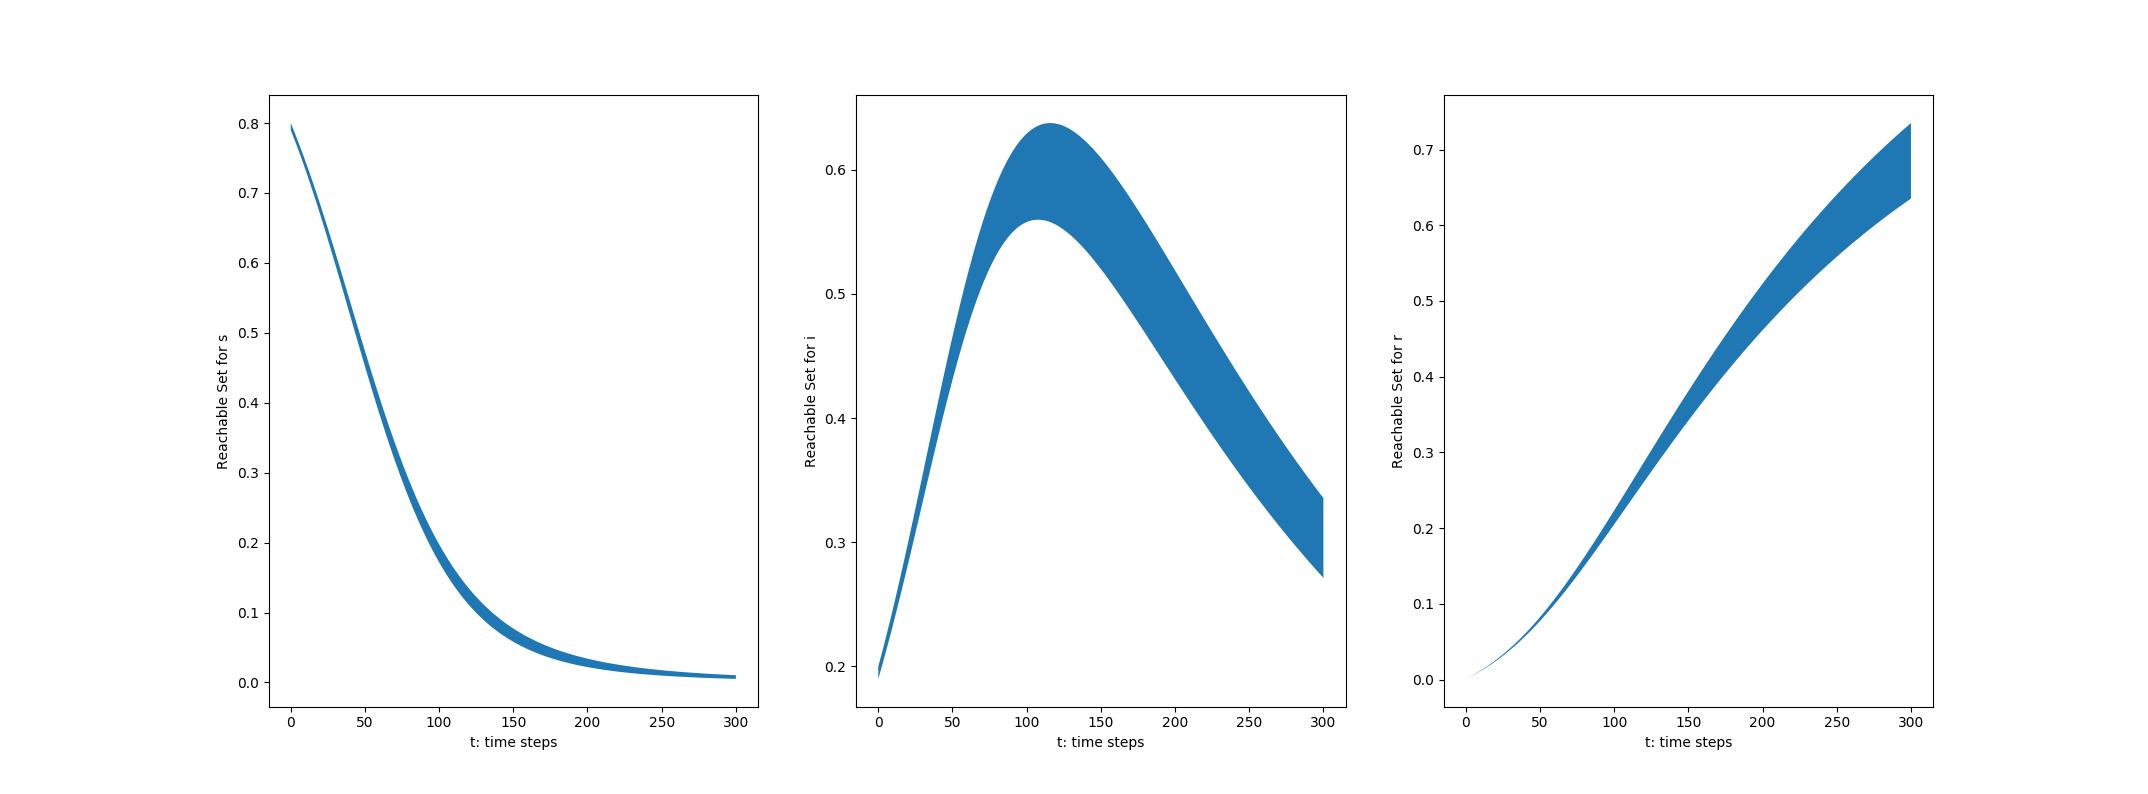
\includegraphics[width=\reachplotwidth\textwidth]{figures/SIRProj.png}
  \caption{Projection of Reachable Set of SIR propagated 300 steps in time.}
  \label{fig:kaa_sir}
\end{figure}

\begin{figure}[h!]
  \hspace*{-2.4cm}
  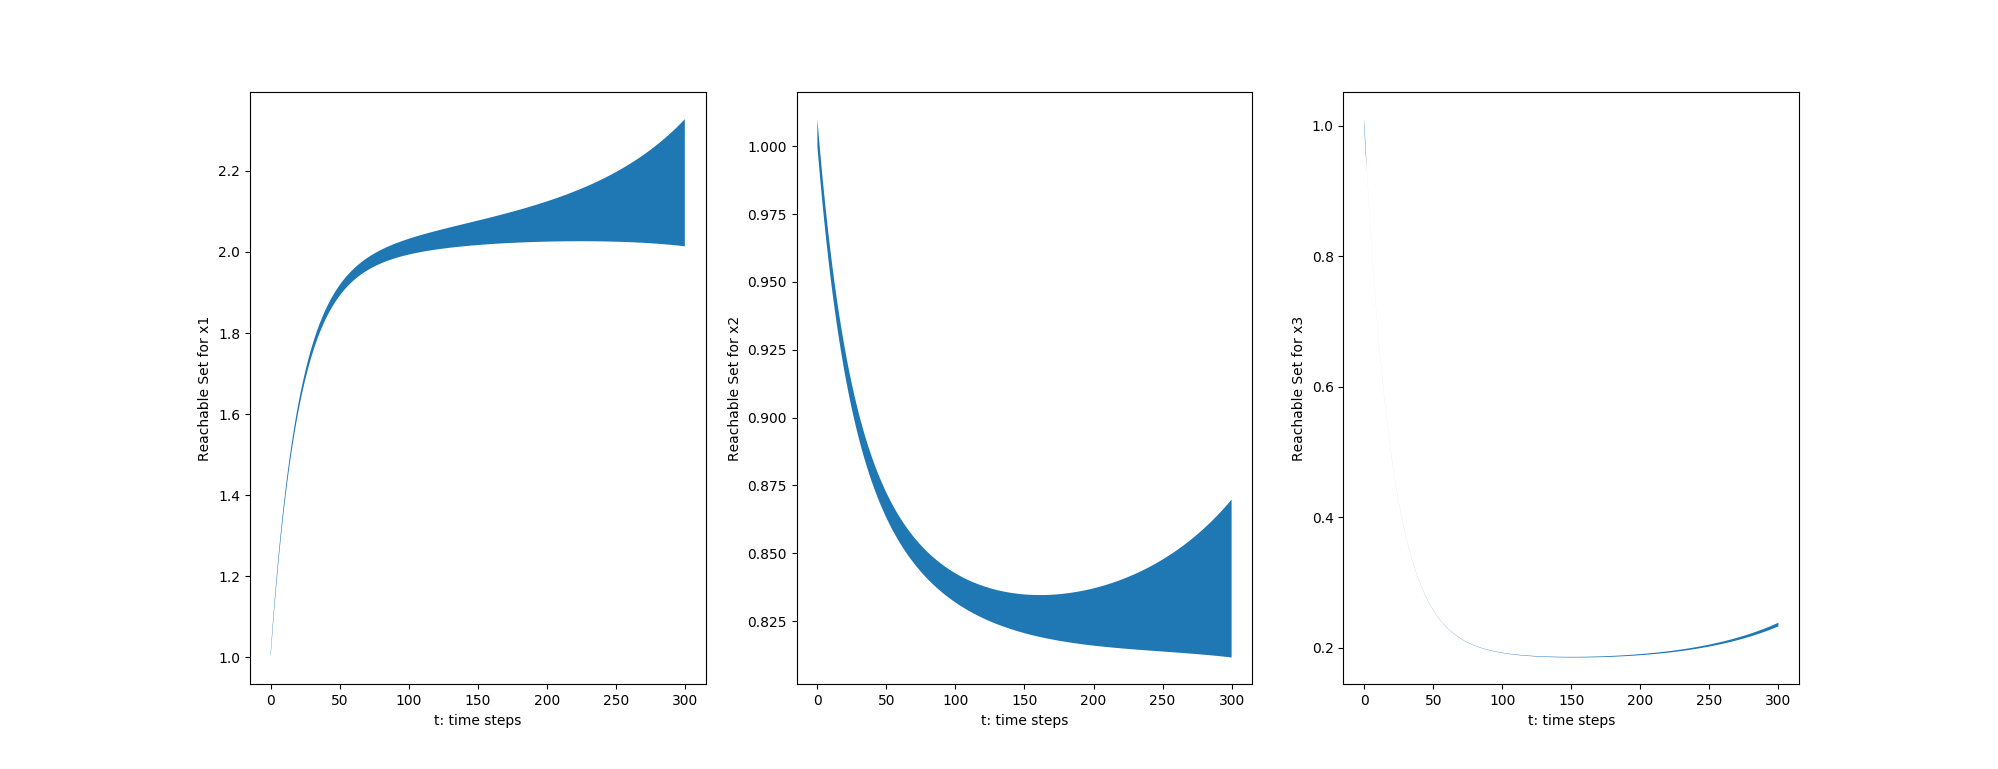
\includegraphics[width=\reachplotwidth\textwidth]{figures/PhosporlayProjOn X_1, X_2, X_3.png}
  \caption{Projection of Reachable Set of the Phosporaley model propagated 300 steps in time.}
  \label{fig:kaa_phos}
\end{figure}
